\documentclass[tikz,border = 10pt]{standalone}
\usetikzlibrary{matrix}
\begin{document}
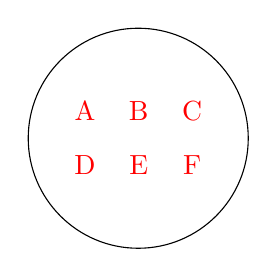
\begin{tikzpicture}
  % commented out: way without matrix library
  %\node[matrix,draw]  {
  %  \node{A}; & \node{B}; & \node{C}; \\
  %  \node{D}; & \node{E}; & \node{F}; \\
  %};
  \matrix[matrix of nodes, draw, circle, nodes= {color = red}] {
    A & B & C \\
    D & E & F \\
  };
\end{tikzpicture}
\end{document}
